\chapter{Les vecteurs (1)}\label{ChLesVecteurs}

\begin{acquis}
\begin{itemize}
\item Connaitre la définition d'un vecteur, du vecteur nul;
\item Connaitre la définition de deux  vecteurs égaux, du milieu d'un segment;
\item Savoir utiliser la règle du parallélogramme, la relation de Chasles pour simplifier une expression comportant des vecteurs;
\item Savoir tracer la somme de deux vecteurs, le produit d'un vecteur par un réel;
\item Savoir montrer que deux vecteurs sont colinéaires.
\end{itemize}
\end{acquis}



\exercicesbase
\begin{colonne*exercice}

\serie{Egalité de vecteurs}

\begin{exercice}
Pour chaque paire de flèches, dire si elles sont le représentant d'un même vecteur ou pas. Justifier vos réponses en termes de : "direction", "sens" et "longueur".

\begin{center}
\definecolor{ffffff}{rgb}{1.,1.,1.}
\begin{tikzpicture}[scale=0.8][line cap=round,line join=round,>=triangle 45,x=1.0cm,y=1.0cm]
\clip(-4.3,-0.42) rectangle (5.76,6.3);
\draw [->] (-3.,5.) -- (-1.,5.);
\draw [->] (-2.,4.) -- (0.,4.);
\draw [->] (2.,5.) -- (4.,5.);
\draw [->] (5.,4.) -- (3.,4.);
\draw [->] (-3.,1.) -- (-2.,3.);
\draw [->] (-3.,1.) -- (-1.,0.);
\draw [->] (2.,2.) -- (5.,2.);
\draw [->] (3.,1.) -- (5.,1.);
\draw (-3.82,5.26) node[anchor=north west] {a)};
\draw (1.2,5.2) node[anchor=north west] {b)};
\draw (-3.76,2.24) node[anchor=north west] {c)};
\draw (1.2,2.22) node[anchor=north west] {d)};
\begin{scriptsize}
\draw [color=ffffff] (-3.,5.)-- ++(-0.5pt,-0.5pt) -- ++(1.0pt,1.0pt) ++(-1.0pt,0) -- ++(1.0pt,-1.0pt);
\draw [color=ffffff] (-1.,5.)-- ++(-0.5pt,-0.5pt) -- ++(1.0pt,1.0pt) ++(-1.0pt,0) -- ++(1.0pt,-1.0pt);
\draw [color=ffffff] (-2.,4.)-- ++(-0.5pt,-0.5pt) -- ++(1.0pt,1.0pt) ++(-1.0pt,0) -- ++(1.0pt,-1.0pt);
\draw [color=ffffff] (0.,4.)-- ++(-0.5pt,-0.5pt) -- ++(1.0pt,1.0pt) ++(-1.0pt,0) -- ++(1.0pt,-1.0pt);
\draw [color=ffffff] (2.,5.)-- ++(-0.5pt,-0.5pt) -- ++(1.0pt,1.0pt) ++(-1.0pt,0) -- ++(1.0pt,-1.0pt);
\draw [color=ffffff] (4.,5.)-- ++(-0.5pt,-0.5pt) -- ++(1.0pt,1.0pt) ++(-1.0pt,0) -- ++(1.0pt,-1.0pt);
\draw [color=ffffff] (5.,4.)-- ++(-0.5pt,-0.5pt) -- ++(1.0pt,1.0pt) ++(-1.0pt,0) -- ++(1.0pt,-1.0pt);
\draw [color=ffffff] (3.,4.)-- ++(-0.5pt,-0.5pt) -- ++(1.0pt,1.0pt) ++(-1.0pt,0) -- ++(1.0pt,-1.0pt);
\draw [color=ffffff] (-3.,1.)-- ++(-0.5pt,-0.5pt) -- ++(1.0pt,1.0pt) ++(-1.0pt,0) -- ++(1.0pt,-1.0pt);
\draw [color=ffffff] (-2.,3.)-- ++(-0.5pt,-0.5pt) -- ++(1.0pt,1.0pt) ++(-1.0pt,0) -- ++(1.0pt,-1.0pt);
\draw [color=ffffff] (-1.,0.)-- ++(-0.5pt,-0.5pt) -- ++(1.0pt,1.0pt) ++(-1.0pt,0) -- ++(1.0pt,-1.0pt);
\draw [color=ffffff] (2.,2.)-- ++(-0.5pt,-0.5pt) -- ++(1.0pt,1.0pt) ++(-1.0pt,0) -- ++(1.0pt,-1.0pt);
\draw [color=ffffff] (5.,2.)-- ++(-0.5pt,-0.5pt) -- ++(1.0pt,1.0pt) ++(-1.0pt,0) -- ++(1.0pt,-1.0pt);
\draw [color=ffffff] (3.,1.)-- ++(-0.5pt,-0.5pt) -- ++(1.0pt,1.0pt) ++(-1.0pt,0) -- ++(1.0pt,-1.0pt);
\draw [color=ffffff] (5.,1.)-- ++(-0.5pt,-0.5pt) -- ++(1.0pt,1.0pt) ++(-1.0pt,0) -- ++(1.0pt,-1.0pt);
\end{scriptsize}
\end{tikzpicture}
\end{center}

\end{exercice}

\begin{exercice}
Donner les caractéristiques des vecteurs suivants en fonction des caractéristiques du vecteur $\overrightarrow{v}$ : \\
\vspace{-5pt}
\begin{tabular}{p{3.5cm}p{3.5cm}}\\
\textbf{a)}$\overrightarrow{a}=\frac{1}{4}\overrightarrow{v}$&\textbf{b)}$\overrightarrow{c}=-\sqrt{5}\overrightarrow{v}$
\end{tabular}
\end{exercice}

\begin{exercice}

On considère les points  A, B, C, D, E et F

placés sur le quadrillage ci-dessous.

\vspace{0.25cm}
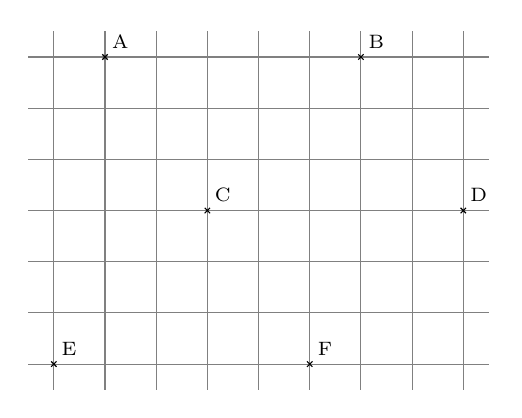
\begin{tikzpicture}[scale=0.65]
\draw [color=gray, xstep=1,ystep=1] (-0.5,-0.5) grid (8.5,6.5);
\begin{scriptsize}
\draw [color=black] (0.,0.)-- ++(-1.5pt,-1.5pt) -- ++(3.0pt,3.0pt) ++(-3.0pt,0) -- ++(3.0pt,-3.0pt);
\draw[color=black] (0.3,0.3) node {E};
\draw [color=black] (5.,0.)-- ++(-1.5pt,-1.5pt) -- ++(3.0pt,3.0pt) ++(-3.0pt,0) -- ++(3.0pt,-3.0pt);
\draw[color=black] (5.3,0.3) node {F};
\draw [color=black] (3.,3.)-- ++(-1.5pt,-1.5pt) -- ++(3.0pt,3.0pt) ++(-3.0pt,0) -- ++(3.0pt,-3.0pt);
\draw[color=black] (3.3,3.3) node {C};
\draw [color=black] (8.,3.)-- ++(-1.5pt,-1.5pt) -- ++(3.0pt,3.0pt) ++(-3.0pt,0) -- ++(3.0pt,-3.0pt);
\draw[color=black] (8.3,3.3) node {D};
\draw [color=black] (6.,6.)-- ++(-1.5pt,-1.5pt) -- ++(3.0pt,3.0pt) ++(-3.0pt,0) -- ++(3.0pt,-3.0pt);
\draw[color=black] (6.3,6.3) node {B};
\draw [color=black] (1.,6.)-- ++(-1.5pt,-1.5pt) -- ++(3.0pt,3.0pt) ++(-3.0pt,0) -- ++(3.0pt,-3.0pt);
\draw[color=black] (1.3,6.3) node {A};
\end{scriptsize}
\end{tikzpicture}


Dire si chacune des égalités suivantes est vraie

ou fausse.

\begin{multicols}{2}[\raggedcolumns]
\begin{enumerate}
\item $\overrightarrow{AB}=\overrightarrow{EF}$
\item $\overrightarrow{CD}=-\overrightarrow{AB}$
\item $\overrightarrow{DA}=\overrightarrow{DB}$
\item $\overrightarrow{ED}=\overrightarrow{BD}$
\item $\overrightarrow{AE}=\overrightarrow{BF}$
\item $\overrightarrow{EF}=-\overrightarrow{DC}$
\end{enumerate}
\end{multicols}
\end{exercice}

\begin{exercice}

\begin{enumerate}
\item Construire un triangle ABC tel que : AB = 3,5 cm, AC = 5 cm et BC = 4 cm.
\item Construire le point D tel que $\overrightarrow{CD}=\overrightarrow{AC}$   et le point E symétrique de B par rapport à C.
\item Quelle est la nature du quadrilatère ABDE ? Justifier votre réponse.
\end{enumerate}

\end{exercice}


\begin{exercice}

Soit ABCD et CDEF deux parallélogrammes.\\
Montrer que ABFE est aussi un parallélogramme.

\end{exercice}

\begin{exercice}
Soit [AB] un segment et I le milieu de [AB].\\
Déterminer dans chaque cas la valeur du réel $\alpha$ pour que l'égalité soit vraie :

\begin{multicols}{2}
\begin{enumerate}

\item $\overrightarrow{AI}=\alpha\overrightarrow{AB}$ ;
\item $\overrightarrow{AI}=\alpha\overrightarrow{IB}$ ;
\item $\overrightarrow{AB}=\alpha\overrightarrow{BI}$ ;
\item $\overrightarrow{AI}+\alpha\overrightarrow{IB}=\overrightarrow{0}$.

\end{enumerate}
\end{multicols}
\end{exercice}

\begin{exercice}
On considère un triangle quelconque $ABS$. On note $A'$ et $B'$ les symétriques respectifs de $A$ et $B$ par rapport à $S$.\\
Que peut-on dire des vecteurs $\overrightarrow{AB}$ et $\overrightarrow{A'B'}$? Justifier votre réponse.
\end{exercice}

\begin{exercice}
\begin{center}
\definecolor{cqcqcq}{rgb}{0.752941176471,0.752941176471,0.752941176471}
\begin{tikzpicture}[line cap=round,line join=round,>=triangle 45,x=1.0cm,y=1.0cm]
\draw [color=cqcqcq,dash pattern=on 2pt off 2pt, xstep=1.0cm,ystep=1.0cm] (-3.54,1.32) grid (3.7,5.66);
\clip(-3.54,1.32) rectangle (3.7,5.66);
\draw (-2.,5.)-- (3.,5.);
\draw (3.,5.)-- (2.,2.);
\draw (2.,2.)-- (-3.,2.);
\draw (-3.,2.)-- (-2.,5.);
\begin{scriptsize}
\draw [color=black] (-2.,5.)-- ++(-0.5pt,-0.5pt) -- ++(1.0pt,1.0pt) ++(-1.0pt,0) -- ++(1.0pt,-1.0pt);
\draw[color=black] (-2.,5.3) node {$A$};
\draw [color=black] (-3.,2.)-- ++(-0.5pt,-0.5pt) -- ++(1.0pt,1.0pt) ++(-1.0pt,0) -- ++(1.0pt,-1.0pt);
\draw[color=black] (-3.02,1.8) node {$B$};
\draw [color=black] (2.,2.)-- ++(-0.5pt,-0.5pt) -- ++(1.0pt,1.0pt) ++(-1.0pt,0) -- ++(1.0pt,-1.0pt);
\draw[color=black] (2.,1.84) node {$C$};
\draw [color=black] (3.,5.)-- ++(-0.5pt,-0.5pt) -- ++(1.0pt,1.0pt) ++(-1.0pt,0) -- ++(1.0pt,-1.0pt);
\draw[color=black] (3.02,5.32) node {$D$};
\end{scriptsize}
\end{tikzpicture}
\end{center}

\begin{enumerate}
\item Reproduire le parallélogramme ABCD ci-dessus puis construire les points E, F, G, H et I définis par :  $\overrightarrow{CE}=\overrightarrow{AC}$;  $\overrightarrow{BF}=\overrightarrow{AC}$;  $\overrightarrow{DG}=\overrightarrow{AC}$ ;  $\overrightarrow{AH}=-\overrightarrow{BC}$ ;  $\overrightarrow{IA}=\overrightarrow{AC}$
\item Quelle est la nature des quadrilatères BCEF et DGEC. Justifier votre réponse.
\item Que représente le point A pour le segment $[IC]$ ?Justifier votre réponse.
\end{enumerate}

\end{exercice}

\newpage

\serie{Opérations sur les vecteurs}

\begin{exercice}

\begin{center}
	\definecolor{qqqqff}{rgb}{0.,0.,1.}
\definecolor{cqcqcq}{rgb}{0.7529411764705882,0.7529411764705882,0.7529411764705882}
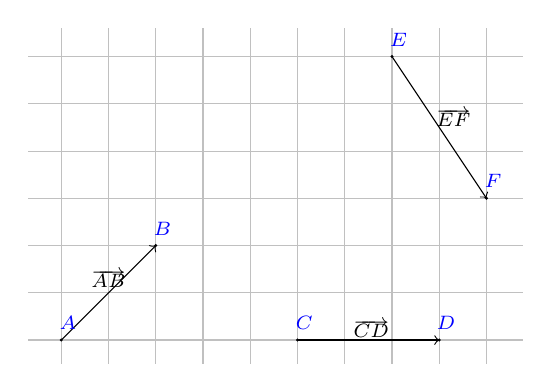
\begin{tikzpicture}[scale=0.6][line cap=round,line join=round,>=triangle 45,x=1.0cm,y=1.0cm]
\draw [color=cqcqcq,, xstep=1.0cm,ystep=1.0cm] (0.3,-3.5) grid (10.78,3.6);
\clip(0.3,-3.5) rectangle (10.78,3.6);
\draw [->] (1.,-3.) -- (3.,-1.);
\draw [->] (6.,-3.) -- (9.,-3.);
\draw [->] (8.,3.) -- (10.,0.);
\begin{scriptsize}
\draw [fill=qqqqff] (1.,-3.) circle (0.5pt);
\draw[color=qqqqff] (1.14,-2.64) node {$A$};
\draw [fill=qqqqff] (3.,-1.) circle (0.5pt);
\draw[color=qqqqff] (3.14,-0.64) node {$B$};
\draw[color=black] (2.,-1.7) node {$\overrightarrow{AB}$};
\draw [fill=qqqqff] (6.,-3.) circle (0.5pt);
\draw[color=qqqqff] (6.14,-2.64) node {$C$};
\draw [fill=qqqqff] (9.,-3.) circle (0.5pt);
\draw[color=qqqqff] (9.14,-2.64) node {$D$};
\draw[color=black] (7.56,-2.76) node {$\overrightarrow{CD}$};
\draw [fill=qqqqff] (8.,3.) circle (0.5pt);
\draw[color=qqqqff] (8.14,3.36) node {$E$};
\draw [fill=qqqqff] (10.,0.) circle (0.5pt);
\draw[color=qqqqff] (10.14,0.36) node {$F$};
\draw[color=black] (9.3,1.7) node {$\overrightarrow{EF}$};
\end{scriptsize}
\end{tikzpicture}
\end{center}

On considère les points $A$, $B$, $C$, $D$, $E$ et $F$ représentés ci-dessus. Reproduire les points et les vecteurs $\overrightarrow{AB}$, $\overrightarrow{CD}$ et $\overrightarrow{EF}$ sur votre cahier. Représenter de plus les vecteurs suivants :\\

\begin{tabular}{p{3.5cm}p{3.5cm}}
\textbf{a)} $\overrightarrow{a}=\overrightarrow{BC}$      & \textbf{e)} $\overrightarrow{e}=\overrightarrow{EF}+\overrightarrow{AB}$  \\\\
\textbf{b)} $\overrightarrow{b}=\overrightarrow{AB}+\overrightarrow{BC}$      & \textbf{f)} $\overrightarrow{f}=\overrightarrow{FE}+\overrightarrow{DC}$  \\\\
\textbf{c)} $\overrightarrow{c}=\overrightarrow{AB}+\overrightarrow{CD}$      & \textbf{g)} $\overrightarrow{g}=\overrightarrow{AB}+\overrightarrow{BC}+\overrightarrow{CD}$ \\\\
\textbf{d)} $\overrightarrow{d}=\overrightarrow{AB}+\overrightarrow{CB}$ 
\end{tabular}

\end{exercice}

\begin{exercice}
Construire un représentant des vecteurs suivants:
\begin{multicols}{2}
\begin{enumerate}
 \item $\overrightarrow{u}+\overrightarrow{AB}$
 \item $\overrightarrow{v}+\overrightarrow{CB}$
 \item $\overrightarrow{w} +\overrightarrow{DE}$
\end{enumerate}
\end{multicols}
   
\definecolor{qqqqff}{rgb}{0.,0.,1.}
\definecolor{cqcqcq}{rgb}{0.752941176471,0.752941176471,0.752941176471}
\begin{tikzpicture}[line cap=round,line join=round,>=triangle 45,x=1.0cm,y=1.0cm]
\draw [color=cqcqcq,dash pattern=on 2pt off 2pt, xstep=1.0cm,ystep=1.0cm] (-2.66,-2.64) grid (5.52,4.18);
\clip(-2.66,-2.64) rectangle (5.52,4.18);
\draw [->] (0.,2.) -- (2.,1.);
\draw [->] (5.,1.) -- (4.,-1.);
\draw [->] (-2.,0.) -- (-1.,1.);
\begin{scriptsize}
\draw [fill=qqqqff] (1.,-1.) circle (1.5pt);
\draw[color=qqqqff] (1.14,-0.72) node {$B$};
\draw [fill=qqqqff] (2.,1.) circle (1.5pt);
\draw[color=qqqqff] (2.14,1.28) node {$C$};
\draw [fill=qqqqff] (4.,2.) circle (1.5pt);
\draw[color=qqqqff] (4.14,2.28) node {$D$};
\draw [fill=qqqqff] (3.,-1.) circle (1.5pt);
\draw[color=qqqqff] (3.14,-0.72) node {$E$};
\draw[color=black] (1.08,1.74) node {$v$};
\draw[color=black] (4.74,0.14) node {$w$};
\draw [fill=qqqqff] (-2.,0.) circle (1.5pt);
\draw[color=qqqqff] (-2.2,0.26) node {$A$};
\draw[color=black] (-1.58,0.78) node {$u$};
\end{scriptsize}
\end{tikzpicture}
\end{exercice}

\begin{exercice}

En utilisant la relation de Chasles, simplifier au maximum les vecteurs suivants :
\begin{enumerate}

\item  $\overrightarrow{u}=\overrightarrow{AB}+\overrightarrow{BC}+\overrightarrow{CE}+\overrightarrow{EG}$
\item $\overrightarrow{w}=\overrightarrow{AB}+\overrightarrow{CB}+\overrightarrow{BD}+\overrightarrow{DE}$
\item  $\overrightarrow{v}=\overrightarrow{AB}+\overrightarrow{DA}+\overrightarrow{CD}+\overrightarrow{BC}$ 
\item $\overrightarrow{n}=\overrightarrow{AG}+\overrightarrow{DE}+\overrightarrow{CD}+\overrightarrow{GC}$

\end{enumerate}
\end{exercice}

\begin{exercice}

Sur chacune des figures suivantes, construire un représentant de $\vec{u}+\vec{v}$ :

\begin{enumerate}
\item \ \

\begin{tikzpicture}[scale=0.7]
\draw [-latex] (0.,0.) -- (4.,1.);
\draw [-latex] (0.,0.) -- (-2.,3.);
\begin{scriptsize}
\draw [color=black,thick] (0.,0.)-- ++(-2pt,-2pt) -- ++(4pt,4pt) ++(-4pt,0) -- ++(4pt,-4pt);
\draw (2,0.5) node[below] {$\vec{u}$};
\draw (-1,1.7) node[above] {$\vec{v}$};
\draw [color=white] (-3,5) circle (1pt);
\draw [color=white] (0,-2) circle (1pt);
\end{scriptsize}
\end{tikzpicture}

\item \ \

\begin{tikzpicture}[scale=0.75]
\draw [-latex] (0.,0.) -- (2.,4.);
\draw [-latex] (-2.,-1.) -- (3.,-2.);
\begin{scriptsize}
\draw [color=black,thick] (0.,0.)-- ++(-2pt,-2pt) -- ++(4pt,4pt) ++(-4pt,0) -- ++(4pt,-4pt);
\draw [color=black,thick] (-2,-1)-- ++(-2pt,-2pt) -- ++(4pt,4pt) ++(-4pt,0) -- ++(4pt,-4pt);
\draw (0.8,2) node[above] {$\vec{u}$};
\draw (0.5,-1.5) node[below] {$\vec{v}$};
\draw [color=white] (-3,3) circle (1pt);
\draw [color=white] (0,-4) circle (1pt);
\end{scriptsize}
\end{tikzpicture}

\end{enumerate}

\end{exercice}

\begin{exercice}
Sur chacune des figures suivantes, construire un représentant de $\vec{u}-\vec{v}$ :

\begin{enumerate}
\item \ \

\begin{tikzpicture}[scale=0.7]
\draw [-latex] (0.,0.) -- (4.,1.);
\draw [-latex] (0.,0.) -- (-2.,3.);
\begin{scriptsize}
\draw [color=black,thick] (0.,0.)-- ++(-2pt,-2pt) -- ++(4pt,4pt) ++(-4pt,0) -- ++(4pt,-4pt);
\draw (2,0.5) node[below] {$\vec{u}$};
\draw (-1,1.7) node[above] {$\vec{v}$};
\draw [color=white] (-3,5) circle (1pt);
\draw [color=white] (0,-2) circle (1pt);
\end{scriptsize}
\end{tikzpicture}

\item \ \

\begin{tikzpicture}[scale=0.75]
\draw [-latex] (0.,0.) -- (2.,4.);
\draw [-latex] (-2.,-1.) -- (3.,-2.);
\begin{scriptsize}
\draw [color=black,thick] (0.,0.)-- ++(-2pt,-2pt) -- ++(4pt,4pt) ++(-4pt,0) -- ++(4pt,-4pt);
\draw [color=black,thick] (-2,-1)-- ++(-2pt,-2pt) -- ++(4pt,4pt) ++(-4pt,0) -- ++(4pt,-4pt);
\draw (0.8,2) node[above] {$\vec{u}$};
\draw (0.5,-1.5) node[below] {$\vec{v}$};
\draw [color=white] (-3,3) circle (1pt);
\draw [color=white] (0,-4) circle (1pt);
\end{scriptsize}
\end{tikzpicture}

\end{enumerate}
\end{exercice}

\begin{exercice}
En utilisant la relation de Chasles, simplifier au maximum les vecteurs suivants :
\begin{enumerate}
\item $\overrightarrow{w}=-\overrightarrow{ED}-\overrightarrow{CB}+\overrightarrow{CD}-\overrightarrow{BA}$\\

\item $\overrightarrow{t}=\overrightarrow{BA}-\overrightarrow{CB}-\overrightarrow{ED}-\overrightarrow{DC}-\overrightarrow{FE}$\\

\item $\overrightarrow{s}=2\overrightarrow{AB}+3\overrightarrow{BC}+\overrightarrow{CD}$\\

 \item $\overrightarrow{n}=-\overrightarrow{BC}-\overrightarrow{DC}+\overrightarrow{DE}+2\overrightarrow{EB}$    \\
 
 \item $\overrightarrow{p}=2\overrightarrow{CD}+10\overrightarrow{DC}+10\overrightarrow{CE}-8\overrightarrow{DE}$ 
 \end{enumerate}
\end{exercice}

\begin{exercice}
Soient $A$, $B$, $C$, $D$ et $E$ des points du plan. En utilisant la relation de Chasles, simplifiez le plus possible les expressions suivantes : 
\begin{enumerate}

\item $\overrightarrow{BC}+\overrightarrow{CD}+\overrightarrow{DE}+\overrightarrow{EF}$    \\\\
\item $\overrightarrow{AB}+\overrightarrow{BC}+\overrightarrow{CD}$ \\\\    
\item $\overrightarrow{EA}-\overrightarrow{EB}-\overrightarrow{CE}-\overrightarrow{BC}$\\\\
\item $2\overrightarrow{AB}-2\overrightarrow{CB}$\\\\
\item $\overrightarrow{AB}+\overrightarrow{CA}+\overrightarrow{BC}$\\\\
 \item $\overrightarrow{AB}+\overrightarrow{EA}+\overrightarrow{BC}+\overrightarrow{CB}$\\\\
 \item $\overrightarrow{AB}-\overrightarrow{ED}-\overrightarrow{DC}+\overrightarrow{EC}+\overrightarrow{BC}$
 
\end{enumerate}
\end{exercice}

\begin{exercice}
Déterminer les caractéristiques des vecteurs suivants par rapport aux caractéristiques du vecteur $\overrightarrow{v}$.\\
\begin{multicols}{2}
\begin{enumerate}
\item $\overrightarrow{a}=-2\overrightarrow{v}$
\item $\overrightarrow{d}=-\overrightarrow{v}$ 
\item $\overrightarrow{b}=3\overrightarrow{v}$
\item $\overrightarrow{e}=\sqrt{2}\overrightarrow{v}$
\item $\overrightarrow{c}=\frac{1}{2}\overrightarrow{v}$
\item $\overrightarrow{f}=-\frac{2}{3}\overrightarrow{v}$  
\end{enumerate}
\end{multicols}
\end{exercice}

\begin{exercice}
\begin{center}
	\definecolor{qqqqff}{rgb}{0.,0.,1.}
\definecolor{cqcqcq}{rgb}{0.7529411764705882,0.7529411764705882,0.7529411764705882}
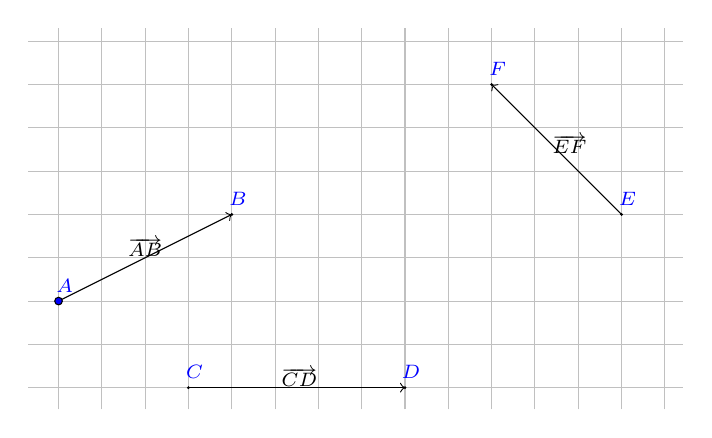
\begin{tikzpicture}[scale=0.55][line cap=round,line join=round,>=triangle 45,x=1.0cm,y=1.0cm]
\draw [color=cqcqcq,, xstep=1.0cm,ystep=1.0cm] (0.3,-4.5) grid (15.42,4.3);
\clip(0.3,-4.5) rectangle (15.42,4.3);
\draw [->] (1.,-2.) -- (5.,0.);
\draw [->] (4.,-4.) -- (9.,-4.);
\draw [->] (14.,0.) -- (11.,3.);
\begin{scriptsize}
\draw [fill=qqqqff] (1.,-2.) circle (2.5pt);
\draw[color=qqqqff] (1.14,-1.64) node {$A$};
\draw [fill=qqqqff] (5.,0.) circle (0.5pt);
\draw[color=qqqqff] (5.14,0.36) node {$B$};
\draw[color=black] (3.,-0.76) node {$\overrightarrow{AB}$};
\draw [fill=qqqqff] (4.,-4.) circle (0.5pt);
\draw[color=qqqqff] (4.14,-3.64) node {$C$};
\draw [fill=qqqqff] (9.,-4.) circle (0.5pt);
\draw[color=qqqqff] (9.14,-3.64) node {$D$};
\draw[color=black] (6.56,-3.76) node {$\overrightarrow{CD}$};
\draw [fill=qqqqff] (14.,0.) circle (0.5pt);
\draw[color=qqqqff] (14.14,0.36) node {$E$};
\draw [fill=qqqqff] (11.,3.) circle (0.5pt);
\draw[color=qqqqff] (11.14,3.36) node {$F$};
\draw[color=black] (12.8,1.62) node {$\overrightarrow{EF}$};
\end{scriptsize}
\end{tikzpicture}
\end{center}
Reporter les vecteurs $\overrightarrow{AB}$, $\overrightarrow{CD}$ et $\overrightarrow{EF}$ sur votre feuille puis représenter les vecteurs suivants :

\begin{multicols}{2}
\begin{enumerate}
\item $\overrightarrow{a}=2\overrightarrow{AB}$ 
\item $\overrightarrow{e}=\overrightarrow{CD}+\overrightarrow{AB}-\overrightarrow{EF}$
\item $\overrightarrow{b}=-\overrightarrow{CD}$
\item $\overrightarrow{f}=\overrightarrow{EF}-\overrightarrow{AB}-\overrightarrow{CD}$
\item $\overrightarrow{c}=\frac{2}{3}\overrightarrow{EF}$
\item $\overrightarrow{g}=2\overrightarrow{AB}+\displaystyle\frac{1}{5}\overrightarrow{CD}$ 
\item $\overrightarrow{d}=\overrightarrow{AB}-\overrightarrow{EF}$
\item $\overrightarrow{h}=\displaystyle\frac{1}{2}\overrightarrow{AB}-\frac{1}{3}\overrightarrow{EF}-\frac{1}{5}\overrightarrow{CD}$
\end{enumerate}
\end{multicols}
\end{exercice}

\begin{exercice}
Soit $ABCD$ un parallélogramme et soit $I$ le milieu de $[DB]$. Compléter les égalités suivantes par un vecteur :
\begin{multicols}{2}
\begin{enumerate}
\item $\overrightarrow{BA}+\overrightarrow{BC}=$
\item $\overrightarrow{IB}+\overrightarrow{ID}=$
\item $\overrightarrow{AI}+\overrightarrow{ID}=$

\end{enumerate}
\end{multicols}
\end{exercice}

\begin{exercice}
On considère un parralélogramme $ABCD$ représenté sur la figure ci-dessous. 
\begin{enumerate}
\item Reproduire la figure puis construire les points $E$ et $F$ tels que $\overrightarrow{DB}=\overrightarrow{AE}$ et $\overrightarrow{BF}=-\overrightarrow{BA}+\overrightarrow{DA}$
\item Montrer que le quadrilatère $ABFE$ est un parallélogramme
\end{enumerate}

\definecolor{zzttqq}{rgb}{0.6,0.2,0.}
\definecolor{qqqqff}{rgb}{0.,0.,1.}
\definecolor{cqcqcq}{rgb}{0.752941176471,0.752941176471,0.752941176471}
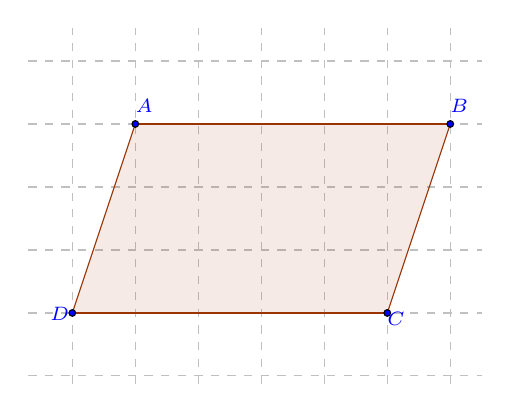
\begin{tikzpicture}[scale=0.8][line cap=round,line join=round,>=triangle 45,x=1.0cm,y=1.0cm]
\draw [color=cqcqcq,dash pattern=on 3pt off 3pt, xstep=1.0cm,ystep=1.0cm] (-2.7,1.88) grid (4.5,7.52);
\clip(-2.7,1.88) rectangle (4.5,7.52);
\fill[color=zzttqq,fill=zzttqq,fill opacity=0.1] (-1.,6.) -- (4.,6.) -- (3.,3.) -- (-2.,3.) -- cycle;
\draw [color=zzttqq] (-1.,6.)-- (4.,6.);
\draw [color=zzttqq] (4.,6.)-- (3.,3.);
\draw [color=zzttqq] (3.,3.)-- (-2.,3.);
\draw [color=zzttqq] (-2.,3.)-- (-1.,6.);
\begin{scriptsize}
\draw [fill=qqqqff] (-1.,6.) circle (1.5pt);
\draw[color=qqqqff] (-0.86,6.28) node {$A$};
\draw [fill=qqqqff] (4.,6.) circle (1.5pt);
\draw[color=qqqqff] (4.14,6.28) node {$B$};
\draw [fill=qqqqff] (3.,3.) circle (1.5pt);
\draw[color=qqqqff] (3.14,2.9) node {$C$};
\draw [fill=qqqqff] (-2.,3.) circle (1.5pt);
\draw[color=qqqqff] (-2.2,2.98) node {$D$};
\end{scriptsize}
\end{tikzpicture}
\end{exercice}

\begin{exercice}
Reproduire la figure ci-dessous  et construire les points définis par les égalités suivantes : 
\begin{multicols}{2}
\begin{enumerate}
\item $\overrightarrow{AB}=3\overrightarrow{AE}$
\item $\overrightarrow{BC}=\frac{1}{2}\overrightarrow{BF}$
\item $\overrightarrow{AG}=\overrightarrow{BA}+2\overrightarrow{BC}$
\end{enumerate}
\end{multicols}

\begin{center}
\definecolor{qqqqff}{rgb}{0.,0.,1.}
\definecolor{cqcqcq}{rgb}{0.7529411764705882,0.7529411764705882,0.7529411764705882}
\definecolor{qqqqff}{rgb}{0.,0.,1.}
\definecolor{cqcqcq}{rgb}{0.752941176471,0.752941176471,0.752941176471}
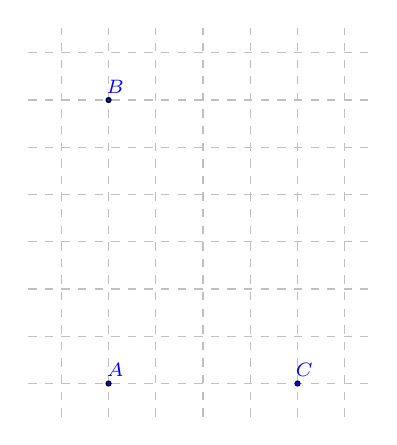
\begin{tikzpicture}[scale=0.6][line cap=round,line join=round,>=triangle 45,x=1.0cm,y=1.0cm]
\draw [color=cqcqcq,dash pattern=on 3pt off 3pt, xstep=1.0cm,ystep=1.0cm] (-2.7,-0.7) grid (4.5,7.52);
\clip(-2.7,-0.7) rectangle (4.5,7.52);
\begin{scriptsize}
\draw [fill=qqqqff] (-1.,0.) circle (1.5pt);
\draw[color=qqqqff] (-0.86,0.28) node {$A$};
\draw [fill=qqqqff] (-1.,6.) circle (1.5pt);
\draw[color=qqqqff] (-0.86,6.28) node {$B$};
\draw [fill=qqqqff] (3.,0.) circle (1.5pt);
\draw[color=qqqqff] (3.14,0.28) node {$C$};
\end{scriptsize}
\end{tikzpicture}
\end{center}
\end{exercice}

\begin{exercice}
Simplifier au maximum les vecteurs suivants :

\begin{enumerate}
\item $\overrightarrow{u}=\overrightarrow{HS}+\overrightarrow{ST}+\overrightarrow{TE}+\overrightarrow{EH}$
\item $\overrightarrow{v}=\overrightarrow{DS}-\overrightarrow{FE}-\overrightarrow{MF}-\overrightarrow{ES}$
\item $\overrightarrow{w}=\overrightarrow{XV}+\overrightarrow{FG}+\overrightarrow{AX}+\overrightarrow{VF}$
\item $\overrightarrow{n}=10\overrightarrow{AG}+3\overrightarrow{GE}-3\overrightarrow{FE}+7\overrightarrow{GF}$    
\end{enumerate}



\end{exercice}

\begin{exercice}
Démontrer les égalités suivantes :
\begin{enumerate}
\item $\overrightarrow{BC}+\overrightarrow{AB}=\overrightarrow{AC}$
\item $\overrightarrow{DH}+\overrightarrow{CK}+\overrightarrow{HC}=\overrightarrow{DK}$
\item $\overrightarrow{AD}-\overrightarrow{CD}-\overrightarrow{AC}=\overrightarrow{0}$
\end{enumerate}

\end{exercice}

\begin{exercice}
On considère $ABCD$ un parallélogramme de centre $O$.\\
Démontrer que :
\begin{enumerate}
\item $\overrightarrow{OC}=\overrightarrow{AC}-\overrightarrow{AO}$
\item $\overrightarrow{BA}+\overrightarrow{DC}=\vec{0}$
\item $\overrightarrow{DB}=\overrightarrow{AB}+\overrightarrow{CB}$
\item $\overrightarrow{AC}=\overrightarrow{DC}+\overrightarrow{BC}$
\end{enumerate}
\end{exercice}

%%%%%%%%%%%%%%%%%%%%%%%%%%%%%%%%%%%%%%%%%%%%%%%%%%%

\serie{Colinéarité}

\begin{exercice}
Soit $ABCD$ un parallélogramme. Soit $I$ le milieu de $[AB]$ et $E$ le point tel que $\overrightarrow{AE}=\frac{1}{3}\overrightarrow{AC}$.
\begin{enumerate}
\item Exprimer $\overrightarrow{AC}$ en fonction de $\overrightarrow{AB}$ et $\overrightarrow{AD}$
\item Exprimer $\overrightarrow{AI}$ en fonction de $\overrightarrow{AB}$
\item Déduire des questions précédentes et de l'énoncé que $\overrightarrow{EI}=\frac{1}{6}\overrightarrow{AB}-\frac{1}{3}\overrightarrow{AD}$
\item Montrer que $\overrightarrow{ED}=-\frac{1}{3}\overrightarrow{AB}+\frac{2}{3}\overrightarrow{AD}$ (une figure n'est \textbf{PAS} une démonstration!).
\item Que peut-on dire des points $E$, $D$ et $I$. Justifier votre réponse.
\end{enumerate}

\end{exercice}


\begin{exercice}

Soit $ABC$ un triangle et $M$ et $N$ les points définis par :
\begin{align*}
\overrightarrow{AM}=3\overrightarrow{AB}-3\overrightarrow{AC} \mbox{ et } \overrightarrow{AN}=\overrightarrow{AB}
\end{align*}
\begin{enumerate}
\item Exprimer $\overrightarrow{CN}$ en fonction de $\overrightarrow{AC}$ et $\overrightarrow{AB}$.
\item Les droites $(CN)$ et $(AM)$ sont-elles parallèles? Justifier votre réponse.
\end{enumerate}

\end{exercice} 


\begin{exercice}

Soient $A$, $B$, $C$ et $D$ quatre points tels que $$3\overrightarrow{AD}=\overrightarrow{AB}+2\overrightarrow{AC}$$
Montrer que les points $B$, $C$ et $D$ sont alignés.

\end{exercice} 

\begin{exercice}

Soient $A$, $B$ et $C$ trois points non alignés.\\
On considère les points $D$ et $E$ tels que :\\
$$\overrightarrow{AD}=\frac{5}{2}\overrightarrow{AC}+\frac{1}{2}\overrightarrow{CB}$$\\
$$\overrightarrow{CE}=-2\overrightarrow{AC}+\frac{1}{2}\overrightarrow{AB}$$\\
Démontrer que les droites $(DE)$ et $(CA)$ sont parallèles.

\end{exercice} 

\begin{exercice}
Soit $OAB$ un triangle.
\begin{enumerate}
	\item Placer les points $C$ et $D$ tels que \\
	$\overrightarrow{OC}=3\overrightarrow{OA}$ et $\overrightarrow{CD}=3\overrightarrow{AB}$
	\item Démontrer que $\overrightarrow{OD}=3(\overrightarrow{OA}+\overrightarrow{AB})$
	\item En utilisant la question précédente, démontrer que les points $O$, $B$ et $D$ sont alignés.
\end{enumerate}
\end{exercice} 

\begin{exercice}
Soit $ABC$ un triangle.
\begin{enumerate}
	\item Placer $D$ et $E$ tels que :\\
$\overrightarrow{CD}=2\overrightarrow{AB}$ et $\overrightarrow{CE}=-3\overrightarrow{AB}$
\item Trouver le nombre $k$ tel que $\overrightarrow{DE}=k\overrightarrow{AB}$. Justifier votre réponse
\item Que peut-on en déduire?
\end{enumerate}
\end{exercice} 

\begin{exercice}
Soit $ABC$ un triangle.\\
On considère les points $D$ et $E$ tels que :\\
$\overrightarrow{AD}=\dfrac{3}{2}\overrightarrow{AB}$ et $\overrightarrow{DE}=\dfrac{3}{2}\overrightarrow{BC}$
\begin{enumerate}
\item Montrer que $\overrightarrow{AE}=\dfrac{3}{2}\overrightarrow{AC}$;
\item Que peut-on en déduire sur les points $A$, $E$ et $C$?
\end{enumerate}
\end{exercice} 

\begin{exercice}
Soit $ABC$ un triangle.\\
On considère les points $M$, $N$ et $P$ tels que :\\
$\overrightarrow{AM}=\dfrac{1}{3}\overrightarrow{AB}$, $\overrightarrow{CN}=\dfrac{1}{3}\overrightarrow{CA}$ et $\overrightarrow{CP}=\dfrac{1}{3}\overrightarrow{BC}$
\begin{enumerate}
\item Montrer que $\overrightarrow{MN}=-\dfrac{1}{3}\overrightarrow{AB}+\dfrac{2}{3}\overrightarrow{AC}$, puis que $\overrightarrow{NP}=\overrightarrow{MN}$;
\item Que peut-on en déduire?
\end{enumerate}
\end{exercice} 

\begin{exercice}
Soit $ABC$ un triangle.\\
On considère les points $E$ et $F$ tels que :\\
$\overrightarrow{AE}=\dfrac{1}{2}\overrightarrow{AB}+\overrightarrow{BC}$ et $\overrightarrow{AF}=\dfrac{3}{2}\overrightarrow{AC}+\overrightarrow{BA}$.
\begin{enumerate}
\item Exprimer $\overrightarrow{EF}$ en fonction de $\overrightarrow{BC}$;
\item Que peut-on en déduire sur les droites $(BC)$ et $(EF)$?
\end{enumerate}
\end{exercice} 

\begin{exercice}
Soit $ABC$ un triangle.\\
On considère les points $D$ et $E$ tels que :\\
$\overrightarrow{BD}=\dfrac{1}{3}\overrightarrow{BC}$ et $\overrightarrow{AE}=\overrightarrow{AC}+2\overrightarrow{AB}$.\\
Montrer que les points $A$, $D$ et $E$ sont alignés.
\end{exercice} 








\end{colonne*exercice}




\connaissances


\QCMautoevaluation{Pour chaque question, plusieurs réponses sont
  proposées.  Déterminer celles qui sont correctes.}


\begin{QCM}

\begin{GroupeQCM}

\begin{center}
\begin{tikzpicture}[scale=0.7][general]
 \draw (0,0)--(1,3)--(3,3)--(2,0)--cycle;
 \draw (1,3)--(3,0)--(5,-0.3)--(3,3);
 \draw (0,0)node[left] {$F$};
 \draw (1,3)node[above] {$A$};
 \draw (3,3)node[above] {$B$};
 \draw (2,0)node[below] {$C$};
 \draw (5,-0.3)node[below] {$D$};
 \draw (3,0)node[below] {$E$};
 \draw[color=C1] (0.5,1.5)node {{\boldmath $\infty$}};
 \draw[color=C1] (2.5,1.5)node {{\boldmath $\infty$}};
 \draw[color=F1] (2,3)node[rotate=90] {{\boldmath $\approx$}};
 \draw[color=F1] (1,0)node[rotate=90] {{\boldmath $\approx$}};
 \draw[color=F1] (4,-0.1)node[rotate=90] {{\boldmath $\approx$}};
\end{tikzpicture}
\end{center}


\begin{exercice}$\overrightarrow{AB}+\overrightarrow{BD}=\overrightarrow{AD}$
\begin{ChoixQCM}{2}
\item vrai
\item faux
\end{ChoixQCM}
\begin{corrige}
\reponseQCM{a}
\end{corrige}
\end{exercice}

\begin{exercice}$AB+BD=AD$
\begin{ChoixQCM}{2}
\item vrai
\item faux
\end{ChoixQCM}
\begin{corrige}
\reponseQCM{b}
\end{corrige}
\end{exercice}

\begin{exercice}$ABDE$ est un parallélogramme.
\begin{ChoixQCM}{2}
\item vrai
\item faux
\end{ChoixQCM}
\begin{corrige}
\reponseQCM{b}
\end{corrige}
\end{exercice}

\begin{exercice}$FCBA$ est un parallélogramme.
\begin{ChoixQCM}{2}
\item vrai
\item faux
\end{ChoixQCM}
\begin{corrige}
\reponseQCM{a}
\end{corrige}
\end{exercice}


\begin{exercice}$\overrightarrow{AB}=\overrightarrow{CF}$
\begin{ChoixQCM}{2}
\item vrai
\item faux
\end{ChoixQCM}
\begin{corrige}
\reponseQCM{b}
\end{corrige}
\end{exercice}

\begin{exercice}$\overrightarrow{DE}=\overrightarrow{BA}$
\begin{ChoixQCM}{2}
\item vrai
\item faux
\end{ChoixQCM}
\begin{corrige}
\reponseQCM{b}
\end{corrige}
\end{exercice}

\begin{exercice}Une expression plus simple de la somme $\overrightarrow{BC}-\overrightarrow{BA}+2\overrightarrow{CD}-\overrightarrow{AD}$ est
\begin{ChoixQCM}{4}
\item $\overrightarrow{CD}$
\item $\overrightarrow{BD}$
\item $\overrightarrow{0}$
\item Autre réponse
\end{ChoixQCM}
\begin{corrige}
\reponseQCM{a}
\end{corrige}
\end{exercice}

\begin{exercice}Un quadrilatère $IJKL$ est un parallélogramme si et seulement si
\begin{ChoixQCM}{4}
\item $\overrightarrow{IJ}=\overrightarrow{KL}$
\item $\overrightarrow{IJ}=\overrightarrow{LK}$
\item $\overrightarrow{IK}=\overrightarrow{JL}$
\item $\overrightarrow{IL}=\overrightarrow{JK}$
\end{ChoixQCM}
\begin{corrige}
\reponseQCM{b,d}
\end{corrige}
\end{exercice}

\begin{exercice}Le point $I$ est le milieu du segment $[AB]$ si et seulement si
\begin{ChoixQCM}{4}
\item $\overrightarrow{AI}+\overrightarrow{IB}=\overrightarrow{AB}$
\item $\overrightarrow{AI}=\overrightarrow{BI}$
\item $\overrightarrow{AI}+\overrightarrow{IB}=\overrightarrow{0}$
\item $\overrightarrow{IA}+\overrightarrow{IB}=\overrightarrow{0}$
\end{ChoixQCM}
\begin{corrige}
\reponseQCM{d}
\end{corrige}
\end{exercice}

\begin{exercice}Si $\overrightarrow{AC}=3\overrightarrow{AB}$ alors 
\begin{ChoixQCM}{3}
\item $\overrightarrow{BC}=2\overrightarrow{BA}$
\item $\overrightarrow{BC}=2\overrightarrow{AB}$
\item $\overrightarrow{CA}=\dfrac{3}{2}\overrightarrow{CB}$
\end{ChoixQCM}
\begin{corrige}
\reponseQCM{b,c}
\end{corrige}
\end{exercice}



\end{GroupeQCM}
\end{QCM}

  




\pagebreak



